Analyzing a massive amount of images requires a better way of handling and sorting them than just storing them into directories. Borrowing ideas of how is the transfer learning process made by the engineers in the Tensorflow team; our catalog system grew to comply with those needs. In a later stage, the analysis process was also included into the system, spawning what could become a framework to analyze visual patterns in sets of images with many different purposes.\\

The development process showed the need for a better set of tools to overcome several difficulties. The training stage involved a repetitive process consisting of manually inspecting the available imagery. To this end, we built a web application on top of our catalog system facilitating this process. The action of continuously showing and tagging images proved to be error-prone, each mistakenly tagged picture, required to log into the database and delete the wrong entry after encoded file names. So a new feature was implemented into our tool, it shows the images and their respective tag and lets the user either delete or edit the classification. Finally, when we had the trained model, and it was predicting on the orthorectified rasters, the ability to geolocate the damaged areas and place them on a map was very convenient.\\


As it was just exposed, we built the application thinking about the final user. Even though the correct implementation from a design perspective is out of the scope of this work, it was exciting to explore it as this would be the kind of problems that arise in the case of getting such a system into production. The last few paragraphs explained how the system grew to a full server-client architecture to respond to the need of processing data and visualizing the results in a meaningful way.\\

The purpose of this chapter is to talk about the implementation of our experiment. We unveil the techniques used to obtain and curate data, and details of the pipeline architecture.\\

\section{Backend}

To understand why some design decision were made we need to understand the nature of our data. Data came in directories taken from the drones and split by flying dates. The quantity and naming of the images were not uniform across towns. Additionally, drone imagery provides metadata that is useful to geolocate the images. However, this information is limited as it only offers the place where the image was taken but gives no information about the image resolution. So the first part of the application was to transform these data into a way that would be easier to manage.\\


Given to previous experience in developing similar projects, we decided to build the system on top of a Python web framework called Django \cite{django}. It offers many solutions out of the box, including a familiar line interface set of commands and an object-relational mapper (ORM) that makes the database integration easier. The feature of being ready to offer a web interface was a great plus.\\


\subsection{Data model}

We took advantage of Django's ORM. It creates Python classes that represent tables in the database and manipulates them as Python objects. In the figure \ref{fig:database} we show a subset of the database diagram. We do not show tables inherent to the features of the Django framework as they were not modified.\\

\begin{figure}[!ht]
  \centering
  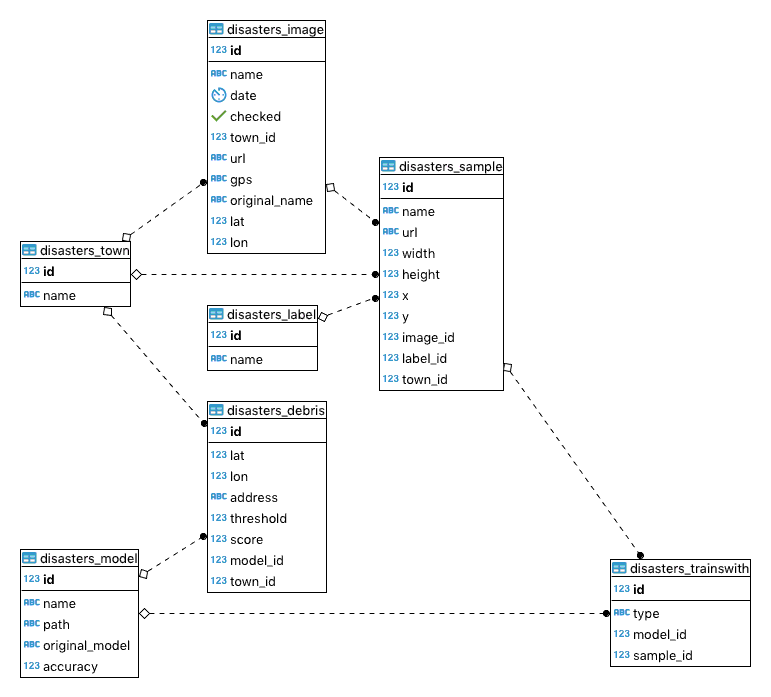
\includegraphics[width=1\textwidth]{images/database.png}
  \caption{Database schema.}
  \label{fig:database}
\end{figure}

We based our database design on reproducible research. It was important to keep track of the characteristics of the models trained as well as the training images used for each model. It was also desirable to be able to reuse models trained with different sets of images for benchmarking. Finally, we wanted to use the best model to predict on the final rasters.\\

\subsection{Ingestion}

We built a process to ingest the images from CENAPRED's FTP. It lazily downloads the images by checking first if the file is already present in the temporary folder, if the file does not exist already, we download it. The system then tries to add it to the database and copies it to the file system. To maintain a coherent one to one mapping between the database and the file system, the process of adding a new scene must be successful both in the database and in the filesystem. Otherwise, we erased the file from both, and the state of the system remains as it was before the ingestion attempt. In Figure \ref{fig:ingest} we show a diagram of this process.\\

\begin{figure}[!h]
  \centering
  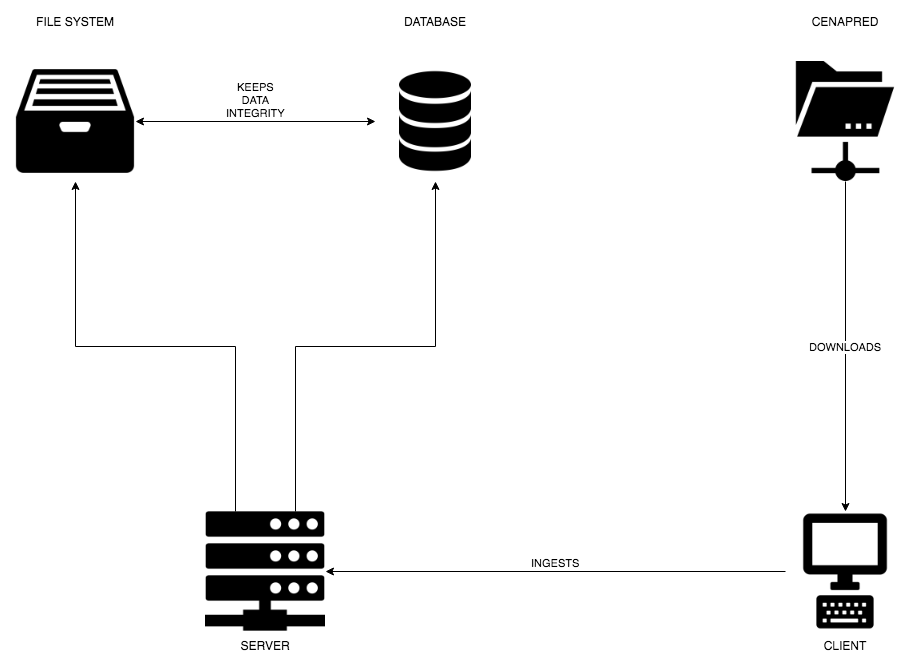
\includegraphics[width=1\textwidth]{images/ingest-diagram.png}
  \caption{We download images from a ftp that CENPRED gave us access to.}
  \label{fig:ingest}
\end{figure}

\subsection{Tagging}

Aerial tagged data is scarce. In particular, for our experiment, we do not have any useful metadata on the images. The idea behind our design was to crowdsource this effort. We built a service that crops samples from the images and exposes them to an online application that lets any user with access to tag an image. We have two categories: the image shows damage, and there is no visible damage in the image. When we obtained a positive answer, the system persists the image in the database with the information about the original image and the coordinates relative to it. In Figure \ref{fig:tag} we show a diagram of this process.\\


\begin{figure}[!h]
  \centering
  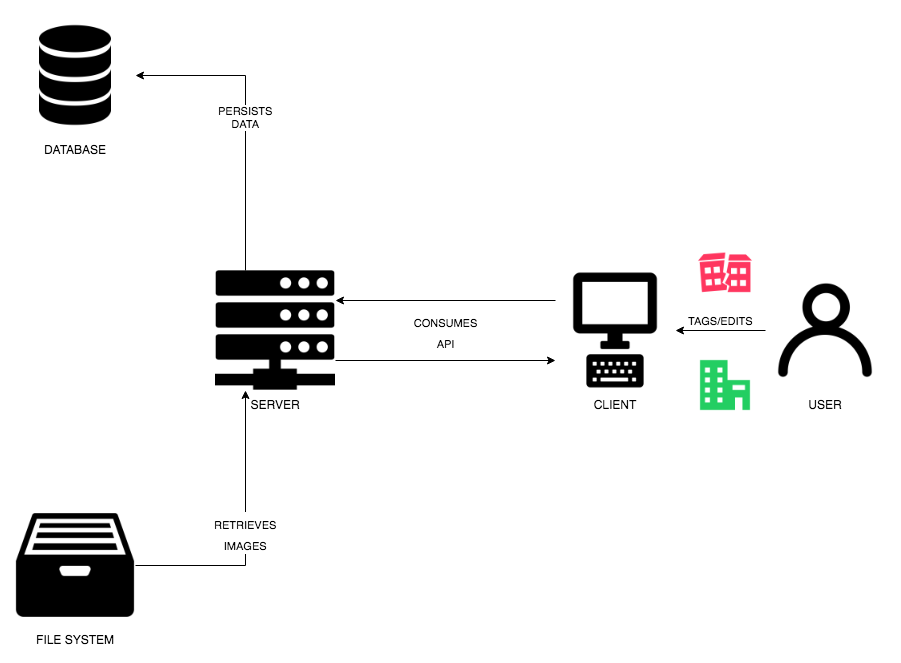
\includegraphics[width=1\textwidth]{images/tag-diagram.png}
  \caption{Tagging process.}
  \label{fig:tag}
\end{figure}


\subsection{Training}

We need to be able to select a sample from the thumbnails that we extracted from the original images. We wanted to create a process that was easily reproductible so we could compare models in a simple fashion. To this end, a random sample is created every time the application runs and the image set is splitted in three sets: training, validation, and testing.\\

The model does not need any geographical information in its training as it relies only on the pixel intensities. We took this to our advantage as we can use the raw drone images for the training stage while predicting on orthorectified mosaics. Tensorflow provides a script for retraining the last layer of Inception by conecting the extracted features into a sofmax layer, and then training this classifier on the given set. It requires a directory layout tailored built to this purpose. We modified and integrated the script into our framework to fit our database design. This process made easier to train several models with similar training, validation, and testing sets. We show a diagram of our process in Figure \ref{fig:train}.\\


\begin{figure}[!h]
  \centering
  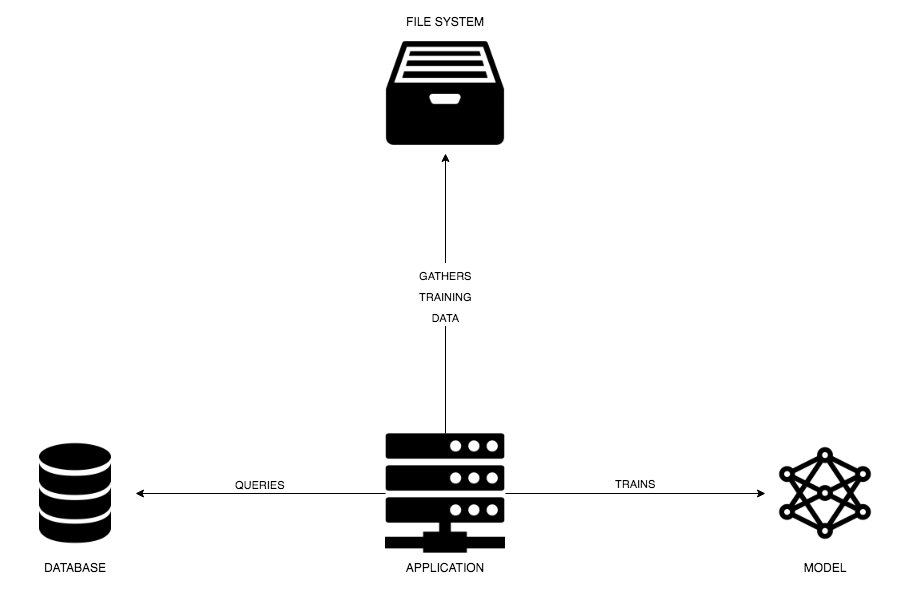
\includegraphics[width=1\textwidth]{images/train-diagram.png}
  \caption{Training process.}
  \label{fig:train}
\end{figure}

\subsection{Prediction}

Although this topic will make more sense once we learn about our experiment results in next chapter, it is worth explaining the process here. Once we have a trained model, we can use it to classify new incoming data and show it to the final user. Once the rasters are subject to the predicting process, results are persisted in the database and the information may be accessible through a client. We show how we ensvision this process in Figure \ref{fig:predict}.\\

\begin{figure}[h]
  \centering
  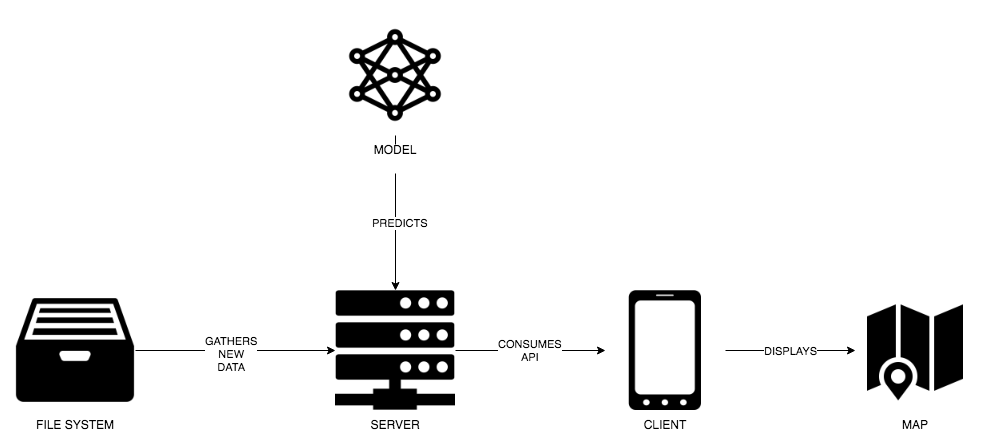
\includegraphics[width=1\textwidth]{images/predict-diagram.png}
  \caption{The system is prepared to predict on new data and display a map with the places in which it founds damaged buildings.}
  \label{fig:predict}
\end{figure}

\section{Frontend}

In the previous section, we talked about the backend components that perform the data governance. At the beginning of the process, we used these components to start our research. However, we soon noticed that it was challenging to manipulate data directly from the file system and the database. To alleviate this inconvenience, we built a set of tools that helped us in this process. This tools were developed using HTML, Javascript and CSS, using a set of common frameworks: Open Layers \footnote{https://openlayers.org/}, Bulma \footnote{https://bulma.io/}, and jQuery \footnote{https://jquery.com/}. While making a full account of the details involved in a web application goes beyond the scope of the present work, we offer a brief description of our tool.\\

\subsection{Data Visualization}

First of all, we needed to know the number of images in the database as well as their geographical location. We developed a view in which we show a map with all the ingested images separated by the town they belong. We also show how many tagged samples have we submitted so far. This view updates each time we add new information to the database. In Figure \ref{fig:visualize} we see the individual views for each of the towns.\\


\begin{figure}[ht]
  \centering
    \begin{subfigure}{.55\textwidth}
        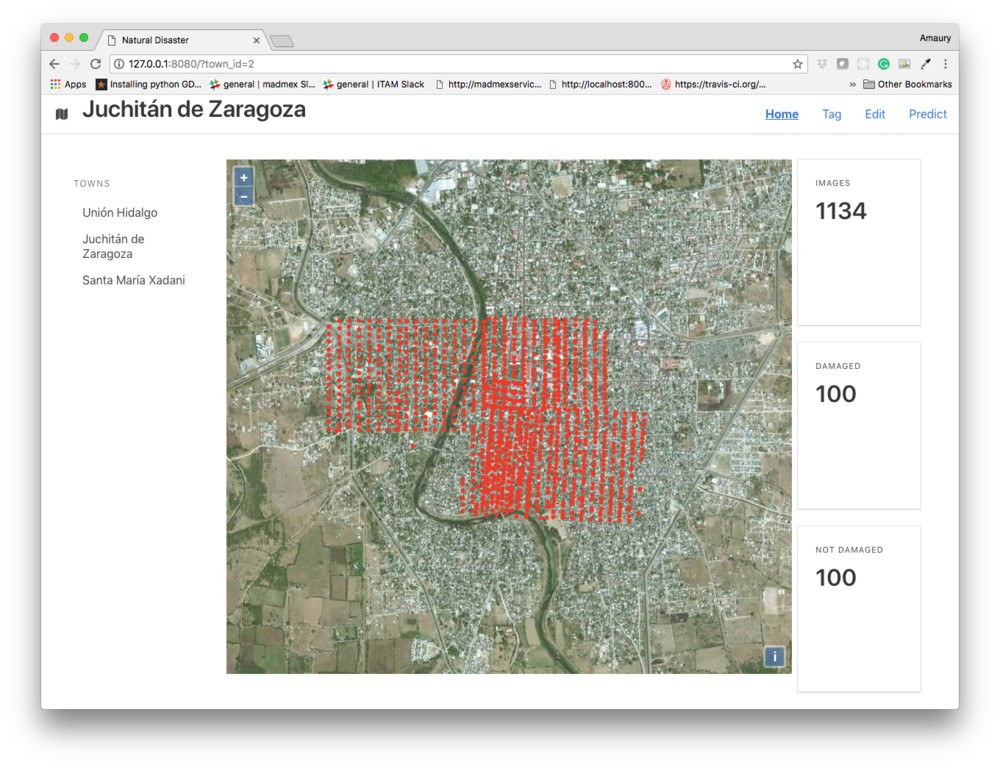
\includegraphics[width=\textwidth]{images/small-app-juchitan.png}
        \caption{Juchit\'an de Zaragoza}
    \end{subfigure}
    \begin{subfigure}{.55\textwidth}
        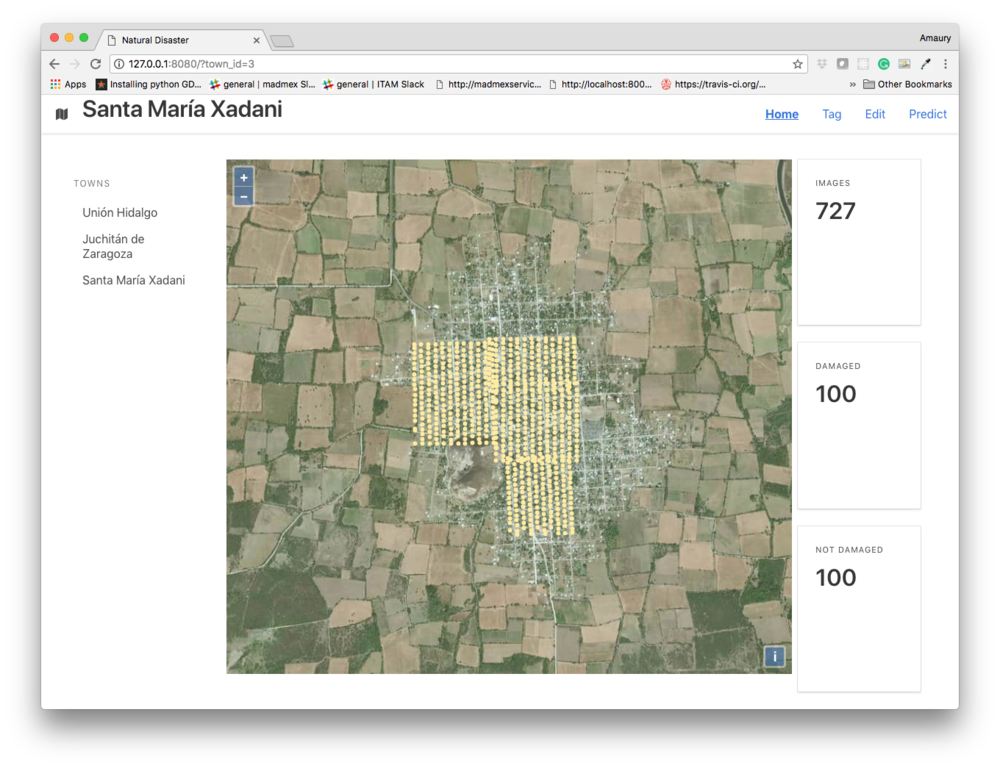
\includegraphics[width=\textwidth]{images/small-app-santamaria.png}
        \caption{Santa Mar\'ia Xadani}
    \end{subfigure}
    %
    \begin{subfigure}{.55\textwidth}
        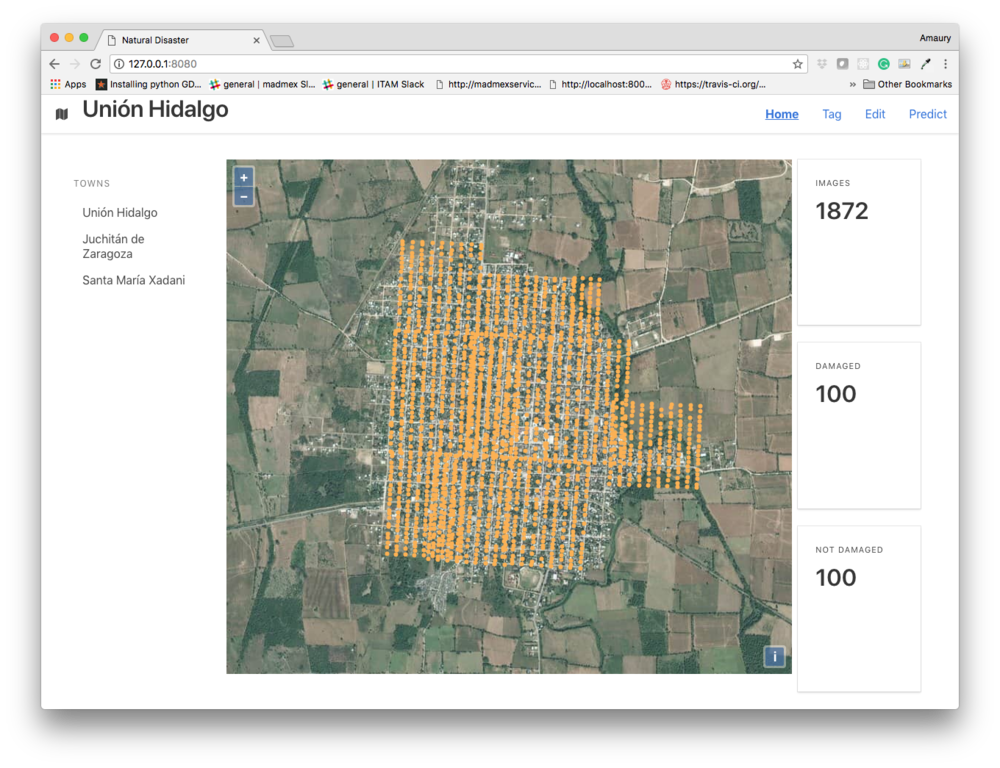
\includegraphics[width=\textwidth]{images/small-app-union.png}
        \caption{Uni\'on Hidalgo}
    \end{subfigure}
  
  \caption{Information interface. We give a summary of the information ingested in the system.}
  \label{fig:visualize}
\end{figure}

\subsection{Tagging}

Cropping and tagging a large number of samples manually from the images was prohibitive, to overcome this obstacle, we developed a unique view for this purpose. The idea was to decentralize the tagging procedure by giving an easy to use tool that was able to run from any browser. This way the cumbersome task of tagging the images could be crowdsourced.\\

A web client was developed using jquery and OpenLayers, and it consumes the endpoints described in the previous section. The interface is an image viewer with a selection and a button to submit an opinion about the highlighted area. In the backend, the image is cropped and ingested into the database assigning the tag that the user selected. In Figure \ref{fig:submit} we see an example of this view.\\


\begin{figure}[!h]
  \centering
  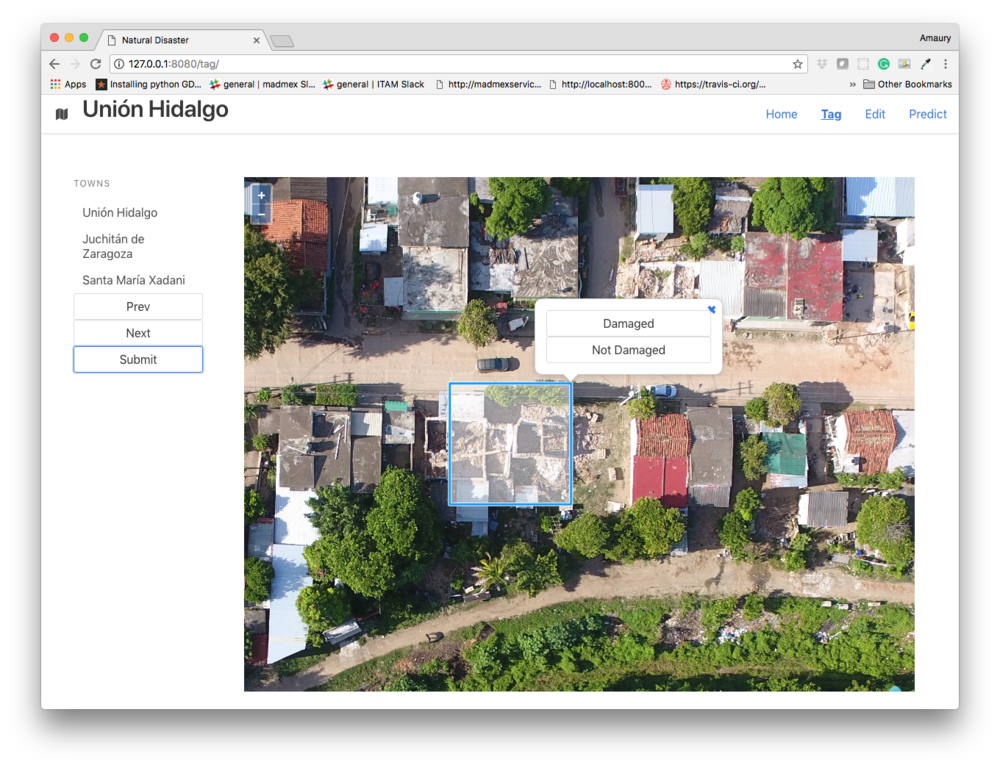
\includegraphics[width=1\textwidth]{images/small-app-tag.png}
  \caption{Submit interface.}
  \label{fig:submit}
\end{figure}

\subsection{Editing}
We noticed that the tagging process was error-prone. In some cases, an image was given an incorrect label, and the error was immediately spotted. To deal with those mistakenly tagged images, we needed to inspect the database and the file system to delete the record. A visualizer for the tagged images was developed to overcome this difficulty. It consists of an interface were the tagged images appear with their respective tag. The interface offers a way to delete or edit the previously assigned tag.\\

\begin{figure}[!h]
  \centering
  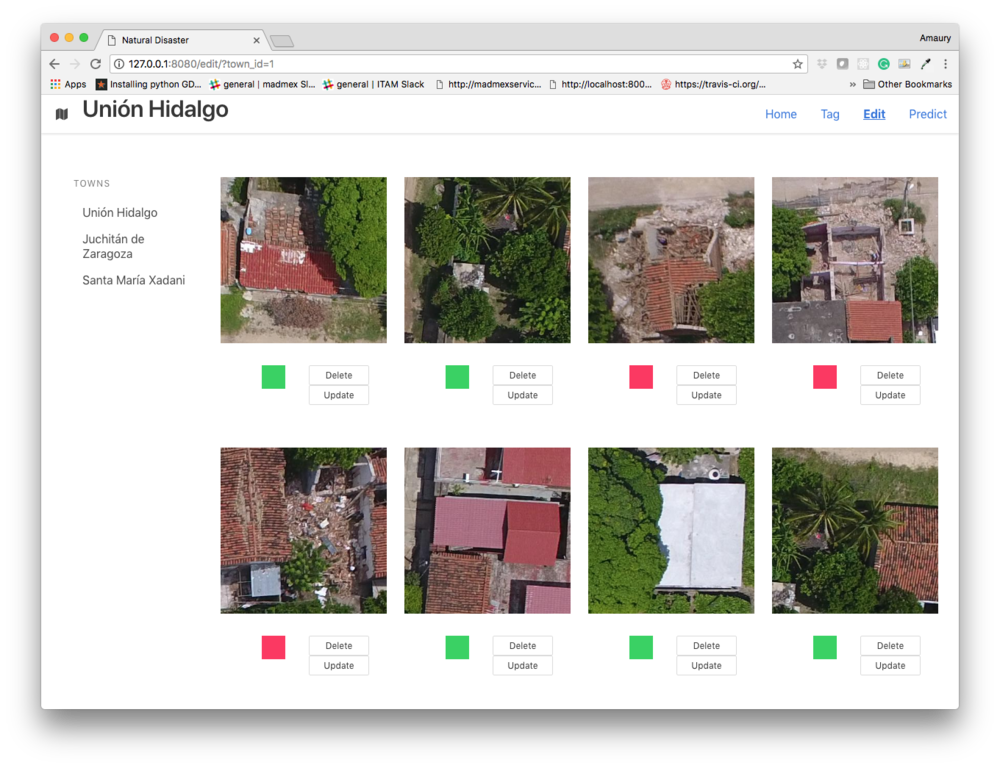
\includegraphics[width=1\textwidth]{images/small-app-edit.png}
  \caption{Edit interface.}
  \label{fig:app-edit}
\end{figure}

\subsection{Predict}

Finally, we developed a view of the points that the algorithm finds in the orthorectified raster. In the final stage of the process, we produced a list of potentially damaged buildings. Those sites also go into the database with geographical information and human readable address obtained from the Google Maps API. We think that this can be helpful to allocate resources most efficiently. Figure \ref{fig:predict} shows how this view looks like.\\

\begin{figure}[!h]
  \centering
  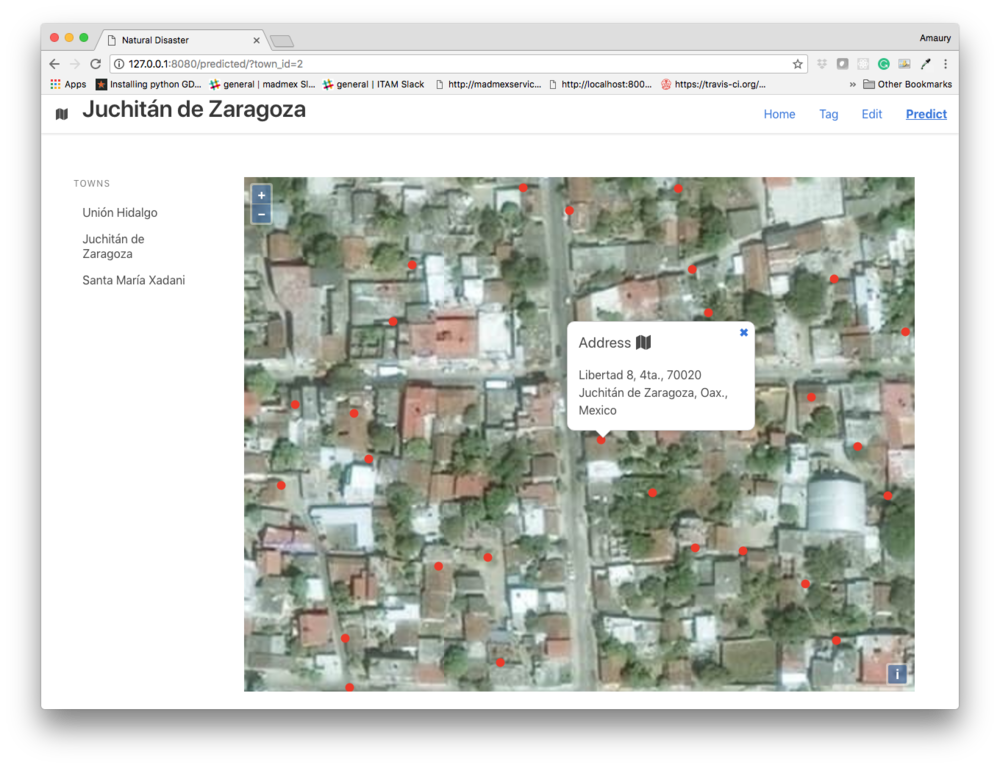
\includegraphics[width=1\textwidth]{images/small-app-predict.png}
  \caption{Predict interface.}
  \label{fig:predict}
\end{figure}


